%% 
%% This is file `sample-sigchi.tex',
%% generated with the docstrip utility.
%%
%% The original source files were:
%%
%% samples.dtx  (with options: `sigchi')
%% 
%% IMPORTANT NOTICE:
%% 
%% For the copyright see the source file.
%% 
%% Any modified versions of this file must be renamed
%% with new filenames distinct from sample-sigchi.tex.
%% 
%% For distribution of the original source see the terms
%% for copying and modification in the file samples.dtx.
%% 
%% This generated file may be distributed as long as the
%% original source files, as listed above, are part of the
%% same distribution. (The sources need not necessarily be
%% in the same archive or directory.)
%%%%%%%%%%%%%%%%%%%%%%%%%%%%%%%%%%%%%%%%%%%%%%%%%%%%%%%%%%%%

%%%%%%%%%%%%%%%%%%%%%%
%%%%%% PREAMBLE %%%%%%
%%%%%%%%%%%%%%%%%%%%%%
\documentclass[sigconf,usenames,dvipsnames,svgnames,table]{acmart}

%% Packages %
  % Standard Packages %
    \usepackage{pdfpages} % Including PDFs. See Graphicx for more info
    \usepackage{amsmath}  % \mvert and other relation symbol
    \usepackage{amssymb}  % Semantic delta=
    \usepackage{amsthm}   % \begin{proof} and related sections
    \usepackage{xspace}   % Spacing for sysname
    \usepackage{dsfont}   % Fancy set letters
    \usepackage{xcolor}   % Things that need attention, and listingsconfig
  % Coding Packages %
    \usepackage{listings}
% \usepackage{sectsty}

\lstdefinelanguage{myC}{
  language=C,
  basicstyle=\ttfamily\singlespacing,
  showspaces=false,              
  showstringspaces=false,        
  showtabs=false,    
  tabsize=2,                      % sets default tabsize to 2 spaces
  captionpos=b,                   % sets the caption-position to bottom
  breaklines=true,                % sets automatic line breaking
  breakatwhitespace=false,
  escapeinside={\%*}{*)},        
  keywordstyle=\bfseries\color{black},    % keyword style
  numberstyle=\tiny\color{gray},
%  numbers=left,
%  frame=single,                  % adds a frame around the code
%  rulecolor=\color{black},
%  stepnumber=1,                 
%  numbersep=5pt,                
%  backgroundcolor=\color{white}, 
%  commentstyle=\color{dkgreen},  % comment style
%  stringstyle=\color{mauve},     % string literal style
}
% A version of the above myC, but without singlespacing
\lstdefinelanguage{myinlineC}{
  language=myC,
  basicstyle=\ttfamily
}
\renewcommand{\ttdefault}{pcr}    % enables bold monospaced font
\lstdefinelanguage[x86gasm]{Assembler}[x86masm]{Assembler}{%
,basicstyle=\ttfamily\singlespacing
,morekeywords={rax,rbx,rcx,rdx,rip,rdi,rsi,rsp,subq,decl,movq
              ,movl,xorl,imull,popq,popl,pushl}%
,morekeywords=[2]{.file,.section,.string,.text,.globl,.cfi_startproc
                 ,.cfi_def_cfa_offset,.cfi_endproc,.size,.ident}%
}
%% \definecolor{cmmtcolor}{named}{DarkGreen}
\definecolor{cmmtcolor}{named}{OliveGreen}
\lstdefinelanguage{Coq}{
,morekeywords={match,end,Definition,Inductive,Lemma,Theorem,Record,
               Hypothesis,Variable,Section,End,case,of,if,then,else,is,let,in,do,return,with,Extract,Constant,Inlined,Inline,Extraction,Fixpoint,Program,Function,Fix,Class,Local,Output,Input}
,morecomment=[s]{(*}{*)}
,keywordstyle=\bfseries\color{MidnightBlue}
,commentstyle={\color{cmmtcolor}}
,basicstyle=\sffamily
,columns=fullflexible
,numberstyle=\tiny\color{gray}
,escapeinside={@}{@}
,literate=
    {:=}{{$\defeq\;$}}1
    {<-}{{$\leftarrow\;$}}1
    {=>}{{$\Rightarrow\;$}}1
    {->}{{$\rightarrow\;$}}1
    {<->}{{$\leftrightarrow\;$}}1
    {<==}{{$\leq\;$}}1
    {\\/}{{$\vee\;$}}1
    {/\\}{{$\land\;$}}1
    {ffun}{{$\mathsf{ffun}$}}1    
    {fun}{{$\lambda$}}1
    {forall}{{$\forall$}}1
    {exists}{{$\exists$}}1
    {Z}{{$\mathbb{Z}$}}1
    {Z0}{{$\mathbb{Z}_0$}}1
    {<=}{{$\leq\;$}}1
    {>=}{{$\geq\;$}}1
    {<>}{{$\neq\;$}}1                
}

%% Verilog
\definecolor{vgreen}{RGB}{104,180,104}
\definecolor{vblue}{RGB}{49,49,255}
\definecolor{vorange}{RGB}{255,143,102}

\lstdefinestyle{verilog-style}
{
    language=Verilog,
    basicstyle=\small\sffamily,
    keywordstyle=\bfseries\color{MidnightBlue},
    identifierstyle=\color{black},
    commentstyle=\color{cmmtcolor},
    tabsize=8,
    moredelim=*[s][\colorIndex]{[}{]},
    literate=*{:}{:}1
}

\makeatletter
\newcommand*\@lbracket{[}
\newcommand*\@rbracket{]}
\newcommand*\@colon{:}
\newcommand*\colorIndex{%
   \edef\@temp{\the\lst@token}%
        \ifx\@temp\@lbracket \color{black}%
            \else\ifx\@temp\@rbracket \color{black}%
                \else\ifx\@temp\@colon \color{black}%
                    \else \color{vorange}%
                        \fi\fi\fi
                        }
\makeatother
                        

    \lstset{language=Coq}
    \usepackage[framemethod=TikZ]{mdframed}
    \mdfsetup{frametitlealignment=\center}
  % Figure Packages %
    \usepackage{caption}  % Captions
    \usepackage{framed}   % Shaded figures
    % \usepackage{epsfig}   % Import PNG figure
    \usepackage{stmaryrd} % Semantics [[ and ]]
  % Specific Thesis Packages %
    \usepackage{contour}
    \usepackage{geometry}
    \usepackage{indentfirst} % Indent after declaring a new (sub)section
    \usepackage[toc,page]
               {appendix} % Add appendix to ToC
    % \usepackage{fontenc}
    % \usepackage{setspace} % Set line spacing
    \usepackage{soul}     % Set highlight colors
    % \usepackage{tocloft}  % Set up Tables of other things
    % \usepackage{fontspec} % Specify Font
    % \usepackage{ragged2e} % Justification
  % Extra %
    % \usepackage{enumitem}
    % \usepackage{tabularx}
    % \usepackage{graphicx}
    % \usepackage{proof}  % To write Proofs (included with amsthm?)

% Custom Colors %
  % For ``shaded'' environments
    \definecolor{MyLightGrey}{gray}{.75}
    \definecolor{shadecolor}{named}{MyLightGrey} 

% Custom Definitions %
  \newcommand{\interp}[1]{\llbracket #1 \rrbracket}
  \newcommand{\shdtt}[1]{\sethlcolor{MyLightGrey}\texttt{\hl{#1}}}
  \newcommand{\obf}[1]{#1^\mathbf{o}}
  \def \sysname {\textsc{G2}\xspace}
  \def \oldname {\textsc{GARUDA}\xspace}
  \def \defeq   {\triangleq}
  \def \bksl    {\textbackslash}
  \def \latex   {\LaTeX\xspace}

%%
%% \BibTeX command to typeset BibTeX logo in the docs
\AtBeginDocument{%
  \providecommand\BibTeX{{%
    \normalfont B\kern-0.5em{\scshape i\kern-0.25em b}\kern-0.8em\TeX}}}

%% Rights management information.  This information is sent to you
%% when you complete the rights form.  These commands have SAMPLE
%% values in them; it is your responsibility as an author to replace
%% the commands and values with those provided to you when you
%% complete the rights form.
\acmConference[]{}{}{}
\setcopyright{acmcopyright}
\copyrightyear{2020}
\acmYear{2020}
% \acmDOI{10.1145/1122445.1122456}

%%
%% Submission ID.
%% Use this when submitting an article to a sponsored event. You'll
%% receive a unique submission ID from the organizers
%% of the event, and this ID should be used as the parameter to this command.
%%\acmSubmissionID{123-A56-BU3}

%%
%% The majority of ACM publications use numbered citations and
%% references.  The command \citestyle{authoryear} switches to the
%% "author year" style.
%% \citestyle{acmauthoryear}

%%
%% end of the preamble, start of the body of the document source.
\begin{document}



%% These commands are for a PROCEEDINGS abstract or paper.
% \acmConference[Woodstock '18]{Woodstock '18: ACM Symposium on Neural
%   Gaze Detection}{June 03--05, 2018}{Woodstock, NY}
% \acmBooktitle{Woodstock '18: ACM Symposium on Neural Gaze Detection,
%   June 03--05, 2018, Woodstock, NY}
% \acmPrice{15.00}
% \acmISBN{978-1-4503-XXXX-X/18/06}

%%
%% The "title" command has an optional parameter,
%% allowing the author to define a "short title" to be used in page headers.
\title{\sysname: a Manuscript}

%%
%% The "author" command and its associated commands are used to define
%% the authors and their affiliations.

%%Check name legality.
\author{Sage Sefton}
\email{ss557415@ohio.edu}
\affiliation{
  \institution{Ohio University}
}

\author{Avinash Karanth}
  \email{karanth@ohio.edu}
\affiliation{
  \institution{Ohio University}
}


%%
%% By default, the full list of authors will be used in the page
%% headers. Often, this list is too long, and will overlap
%% other information printed in the page headers. This command allows
%% the author to define a more concise list
%% of authors' names for this purpose.
\renewcommand{\shortauthors}{Sefton and Karanth}

\begin{abstract}

Runtime monitors to enforce processor security policies are a widely researched field.
Many systems tackle particular issues such as non-interference, cache side-channel attacks, or speculation exploits \cite{2017secverilogbl, 2019stt}.
As the attack model is ever-mutating and often undetected, these solutions can only ever solve part of the problem.
Some solutions propose generic monitors based on programmable hardware monitors \cite{2014pump} or languages for describing arbitrary policies \cite{2018garuda, 2014netkat}.
We build on the idea of verifiable policy design and empower \oldname to support Speculative and Out-of-Order Processors.
The benefits of Speculative and OOP microarchitectures are one of the most significant advancements in recent latency-mitigation research.
\sysname benefits from a refined information model and taint tracking, implemented without changes to the language itself.
These additions incur marginal processor overhead, and ring true to the spatial and power efficiency goals of the past.
We inject monitors into only one part of the processor and automate the comparator for a more streamlined design.
Finally, we will release this code, compiler, and language on GitHub.

\end{abstract}

%%%%%%%%%%%%%%%%%%%%%%%%%
%%% BEGIN             %%%
%%% TABLE OF CONTENTS %%%
%%%%%%%%%%%%%%%%%%%%%%%%%
%%% This will probably be removed at a later date,
%%% but it allows for easier navication now.
  \addcontentsline{toc}{section}{Contents}
  \tableofcontents
%%%%%%%%%%%%%%%%%%%%%%%%%
%%% END               %%%
%%% TABLE OF CONTENTS %%%
%%%%%%%%%%%%%%%%%%%%%%%%%

%%
%% The code below is generated by the tool at http://dl.acm.org/ccs.cfm.
%% Please copy and paste the code instead of the example below.
% %%
% \begin{CCSXML}
% <ccs2012>
%    <concept>
%        <concept_id>10010583.10010717.10010721</concept_id>
%        <concept_desc>Hardware~Functional verification</concept_desc>
%        <concept_significance>500</concept_significance>
%        </concept>
%    <concept>
%        <concept_id>10010583.10010682.10010689</concept_id>
%        <concept_desc>Hardware~Hardware description languages and compilation</concept_desc>
%        <concept_significance>300</concept_significance>
%        </concept>
%    <concept>
%        <concept_id>10010583.10010786.10010787.10010789</concept_id>
%        <concept_desc>Hardware~Emerging languages and compilers</concept_desc>
%        <concept_significance>500</concept_significance>
%        </concept>
%    <concept>
%        <concept_id>10010520.10010521.10010522.10010526</concept_id>
%        <concept_desc>Computer systems organization~Pipeline computing</concept_desc>
%        <concept_significance>100</concept_significance>
%        </concept>
%    <concept>
%        <concept_id>10002978.10003001.10003002</concept_id>
%        <concept_desc>Security and privacy~Tamper-proof and tamper-resistant designs</concept_desc>
%        <concept_significance>500</concept_significance>
%        </concept>
%    <concept>
%        <concept_id>10002978.10003001.10003599.10011621</concept_id>
%        <concept_desc>Security and privacy~Hardware-based security protocols</concept_desc>
%        <concept_significance>500</concept_significance>
%        </concept>
%  </ccs2012>
% \end{CCSXML}

% \ccsdesc[500]{Hardware~Functional verification}
% \ccsdesc[300]{Hardware~Hardware description languages and compilation}
% \ccsdesc[500]{Hardware~Emerging languages and compilers}
% \ccsdesc[100]{Computer systems organization~Pipeline computing}
% \ccsdesc[500]{Security and privacy~Tamper-proof and tamper-resistant designs}
% \ccsdesc[500]{Security and privacy~Hardware-based security protocols}

%%
%% Keywords
\keywords{hardware security, software verification, memory obfuscation}

%%
%% This command processes the author and affiliation and title
%% information and builds the first part of the formatted document.
\maketitle
%%%%%%%%%%%%%%%%%%%%%%%
%%% BEGIN SECTION 1 %%%
%%% INTRODUCTION    %%%
%%%%%%%%%%%%%%%%%%%%%%%
  \section{Introduction}\label{sec:intro}
    \sysname Intro
    \cite{2011gem5sim}
    \cite{2019stt}
    This manuscript loosely follows a standard academic journal's organization.
    Section~\ref{sec:priorwork} summarizes a prior attack models and their proposed solutions.
    The \sysname language is described in detail in Section~\ref{sec:spec} and is demonstrated in Section~\ref{sec:proofs}.
    Section~\ref{sec:compile} describes the intermediate steps towards the compilation of \sysname into Verilog.
    Research done since this paper's release are shown in Section~\ref{sec:more}.
    Sections~\ref{sec:conclude} and~\ref{sec:coauthor} conclude and cite the work done by my colleagues and advisors.
%%%%%%%%%%%%%%%%%%%%%
%%% END SECTION 1 %%%
%%% INTRODUCTION  %%%
%%%%%%%%%%%%%%%%%%%%%

%%%%%%%%%%%%%%%%%%%%%%%
%%% BEGIN SECTION 2 %%%
%%% PRIOR WORK      %%%
%%%%%%%%%%%%%%%%%%%%%%%
  \section{Prior Work}\label{sec:priorwork}
    All the prior work we have seen seems to fall under two broad categories: runtime monitors, or compile-time verification.
    Runtime monitors are sometimes programmable after synthesis, making them more dynamic for general applications.
    They can make decisions on how to enforce a policy while the processor is actively executing instructions.
    Compiler extensions and verification tend to be static.
    The user cannot change the enforced policy after the IC has been synthesized.
    However, compiler extensions also tend to have less temporal, spatial, and energetic overhead than their runtime counterparts.
    The synthesized processor does not trap when a compiled policy is violated.
    Rather, it simply cannot execute prohibited instructions. 
    A comparison of the two can be found in Table~\ref{table:prior:run-vs-comp}.
    In Section~\ref{sec:spec}, %%TODO: point to subsection?
    we will see how \sysname fits into this classification.

    \subsection{Runtime Monitors}\label{sec:prior:runtime}
      As discussed above, a popular angle of attack for protecting computer hardware is the insertion of a runtime monitor.
      These monitors may be static~\cite{2010trustnetdatawatch} or programmable~\cite{2007raksha, 2014pump}.
      There are three publications on this subject that we studied before writing \sysname.

      \subsubsection{TrustNet and DataWatch}\label{sec:prior:runtime:tndw}
        In the 2010 publication, \textit{Tamper Evident Microprocessors}~\cite{2010trustnetdatawatch}, \textbf{TrustNet} and \textbf{DataWatch} were introduced as a pair of complementary monitors.
        The aim of these monitors is to detect hardware trojans within the system they are implemented in.
        The attack model revolves around the possibilities of a malicious engineer inserting a tampered functional unit, or a simple mistake that was not patched before synthesis.
        Rather than use the older solutions that rely on duplication, they call attention to a basic principle of all microprocessors.
        For any given functional unit (\textit{Fetch, Execute, Memory}), the execution of an instruction is separate, but not independent, of the actions of the surrounding units.
        For example, the execution of an arithmetic instruction in the \textit{EXE} stage of a pipeline occurs at a later time than accessing the arguments from the \textit{Register File (RF)}.
        This is to say, the action of gathering arguments and then executing the instruction are two separate events.
        However, how the \textit{EXE} unit behaves is directly dependent on what happens in the \textit{RF}.
        With this observation, \textbf{TrustNet} can determine if a functional unit is behaving erratically.
        The behavior of each unit can be predicted by its inputs, and a mismatch in the prediction and performed actions indicates potentially dishonest programming.
        \par

        A keen reader will have noticed that if multiple functional units have been tampered with, \textbf{TrustNet} may be unable to detect inconsistencies.
        The publishers note that previous research suggests this to be near-infeasible, and carry on with the assumption that only one unit has been altered.
        \par

        \textbf{DataWatch} is a simpler idea that focuses on memory accesses.
        Suppose the tampered \textit{MEM} stage does not attempt to execute multiple instructions from one, but instead tries to redirect the storage of a secret to an insecure location.
        \textbf{DataWatch} protects against these kinds of attacks with partial duplication of the data cache.
        If a store is fired to save at $\$(01)$ but the \textit{MEM} unit attempts to save to $\$(05)$, \textbf{DataWatch} can detect this discrepancy.
        It should be noted that a full duplication of the cache is not practical, so cache mapping techniques are employed.
        However, incomplete mappings of the original cache to the reference cache may allow for small holes in their detection net.

      \subsubsection{Raksha and PUMP}\label{sec:prior:runtime:RP}
        These two programmable monitors are actually different publications, but they are similar enough to be discussed in tandem.
        Indeed, \textit{Raksha} is cited as a reference in \textit{PUMP}~\cite{2014pump, 2015pumpupol}, and that citation is how I originally came across the technology.
        \textit{PUMP}~\cite{2014pump} is a Programmable Unit for Metadata Processing (hence the name).
        They add a new stage to the standard 5-stage pipeline, the namesake programmable unit.
        The authors were clearly fans of Isaac Asimov's \textit{The Gods Themselves}~\cite{1972tgt} in which another one of his many computational rules is introduced.
        The $0-1-\infty$ rule, in short, states that there should not be arbitrary constraints put on standards or rulesets.
        An action should be disallowed, allowed once, or allowed to reoccur indefinitely.
        For contrast, assume a theoretically perfect printer that will never break.
        If it allows only 100 prints, it would violate the $0-1-\infty$ rule as there is an arbitrary constraint on what the user can do.
        \textit{PUMP} follows this rule by allowing an arbitrary number of policies to be defined.
        They cleverly implement this by use of a policy cache that stores ``concrete rules'' and the ability to define policies as ``symbolic rules''.
        Symbolic rules can be nested like parenthetical expressions, but they always compile to the concrete rules used in the cache.
        This ``compilation'' is done dynamically whenever the \textit{PUMP} determines the need for another concrete rule.
        It simply looks at the set of symbolic rules and unravels them until it hits the concrete floor.
        \par

        \textit{Raksha}~\cite{2007raksha} is indirectly crtiticized in \textit{PUMP} for not honoring the $0-1-\infty$ rule.
        However, it is still worth taking a look at.
        As an interesting side note, \textit{Raksha} is reported to mean \textit{protection} in Sanskrit.
        \textit{Raksha} benefits in comparison to \textit{Gate-Level Information Flow Tracking} (GLIFT)~\cite{2009glift} because it does not require a full duplication set of the gates.
        Ironically, \textit{Raksha} was published two years prior to GLIFT.
        \textit{Raksha} follows the idea of Dynamic Information Flow Tracking (DIFT) to provide ``a \textit{flexible and programmable mechanism for specifying security policies}''~\cite{2007raksha} (emphasis theirs).
        They also enable the ability for exceptions to resolve at the same level of the violating program; the core of why I discuss this solution.
        \par

        Many security monitors, programmable or otherwise, determine their actions at the Operating System (OS) level.
        The OS level is generally avoided as mush as possible, as there are no restrictions on what the OS can do.
        This is by definition of the OS itself, and is why the \shdtt{sudo} command exists in most shells.
        You can tell the \shdtt{root} (lowest level) to do something without going into the \shdtt{su} (superuser).
        The ability to write a command like \shdtt{sudo apt-get install gcc} helps avoid accidents if the user types \shdtt{rm \bksl} immediately afterwards.
        However, the OS will not allow itself to be deleted by a lower process and \shdtt{rm \bksl} would fail in any protected terminal.
        For most processes, a form of sandboxing is implemented.
        This means they cannot alter the memory space of external or higher processes.
        In reality, the implementation for many apps is a bit more complicated to allow for controlled inter-application communication.
        \par

        \textit{Raksha}, in the same spirit, processes violations in the same security space as the offending program.
        Preventing traps to the OS, or a similarly powerful process, prevents attacks that exploit this trapping.
        If a process can manage to deduce how such a trap occurs, it may be able to exploit it.
        If the reader knows what SQL Injection Attacks are, they will be all too familiar with this idea.
        A poorly constructed trap, even good systems, can have injection attacks.
        In addition, it should be noted that a trap is generally a very slow event.
        \textit{Raksha} also uses program-level resolution to increase the speed of the entire system.
        Their implementation on an FPGA demonstrates this nicely.

    \begin{table}
      \centering
      \begin{tabular}{|c|l|l|} 
        \hline
          & Rumtime Monitors & Compiler Enforcements\\
        \hline
          Advantages
          & - Often programmable 
            & - Low Overhead \\
          & - Can trigger exceptions or
            & - Possible violations detected \\
          &\quad OS traps &\quad before synthesis \\ 
          & - Modular, not application  
            & - Violations during runtime \\
          &\quad specific &\quad simply fail \\
          \hline
          Disadvantages
          & - Exceptions and traps are slow 
            & - Static after synthesis \\
          & - Larger overhead 
            & - Violation-response is static \\
          & &\quad and defined at compile time \\
        \hline
      \end{tabular}
      \caption{Comparison of Runtime Monitors and Compile-Time Enforcement.}
      \label{table:prior:run-vs-comp}
    \end{table}

    \subsection{Verilog Extensions}\label{sec:prior:csbl}
      Verilog extension research is vast, but this thesis will focus on a chain of four very similar ones ~\cite{2011caisson, 2014sapper, 2015secverilog, 2017secverilogbl}.
      Each of these verilog extensions is fairly incremental, and they all work to enforce security lattices in the hardware code itself.
      As mentioned earlier and demonstrated in Table~\ref{table:prior:run-vs-comp}, these solutions are static once fabricated.
      As you will see though, they manage to implement their goals well within this restriction.

      \subsubsection{Caisson}\label{sec:prior:csbl:c}
        In short, \textit{Caisson}~\cite{2011caisson} will not allow an instruction to access a part of the hardware if it does not meet the required security level.
        The authors define a Verilog extension to facilitate assigning hardware modules different security levels.
        Two levels of security are defined, \textit{high} (H: trusted), and \textit{low} (L: untrusted).
        When defining a module, the compiler makes the user apply a security tag (H or L).
        This solution alone would closely resemble the spatial efficiency pitfalls of GLIFT~\cite{2009glift}.
        In response to this problem, \textit{Caisson} allows nested and parameterized security levels.
        In short, the engineer does not have to copy each module for each security level.  The compiler takes care of that, and introduces efficiency fixes.
        I recommend looking at Figure 2 of their paper to get a better idea of how to code using these nesting and parameterizing features.

      \subsubsection{Sapper}\label{sec:prior:csbl:s}
        An improvement on \textit{Caisson}, \textit{Sapper}~\cite{2014sapper} is largely composed by the same authors.
        The main contribution of this paper is that registers and wires can be connected to the security levels as well.
        They also provide an in-depth description of the type-checking in their compiler.
        Taint tracking is much easier to implement in \textit{Sapper} than in their previous work, so they demonstrate their additions with this example.
        Taint tracking is a method of tracking the propagation of insecure data manipulation.
        An insecure process may attempt to alter a secure segment of memory.
        This can have cascading effects on other, indirectly altered data.
        Tainting the result of any tainted instruction or argument is an effective way of determining if a piece of data has been compromised.
        In addition to this variability, improved \textit{state transitions} are introduced.
        In \textit{Caisson}, the engineer could add what are effectively branches and return systems to their code, something not seen within standard synthesizable Verilog.
        Sapper extends these keyword calls with their mutable tagging system. 

      \subsubsection{SecVerilog and SecVerilog BL}\label{sec:prior:csbl:sv}
        \textit{SecVerilog}~\cite{2015secverilog} and its extension \textit{SecVerilogBL}~\cite{2017secverilogbl} are authored by a different university with different people.
        However, they cite, and seem to continue the work of, both \textit{Caisson} and \textit{Sapper}.
        \textit{SecVerilog} starts by enforcing time-sensitivity and enables significantly more complex security policies.
        Recall \textit{PUMP} from Section~\ref{sec:prior:runtime:RP} and the ability to dynamically track information and security policies using symbolic rules.
        In the same vein, \textit{SecVerilog} enables a user to write dynamic security lattices.
        This non-concrete method of enforcing a lattice is not possible in \textit{Caisson} or \textit{Sapper}.
        \par

        \textit{SecVerilogBL} improves upon its predecessor in a few ways.
        For convenience, there can be multiple security levels assigned to a single variable.
        This is achieved by enabling security tagging at the bit level and for each element of an array.
        For example, the user could assign the lower half of a word to low security, and the upper half to higher security.
        More importantly, they extend \textit{SecVerilog} by adding the ability to downgrade a piece of data.
        They use this new method sparingly, but demonstrate how it can improve the security of previously unprotected level-changing techniques.
        In fact, of all the solutions mentioned so far in Section~\ref{sec:prior:csbl}, only \textit{SecVerilogBL} seems to have an intuitive way for the user to declassify elements.

    \subsection{Kleene Algebras}\label{sec:prior:ka}
      While not exclusive to security, I would like to explain the core of Kleene Algebra~\cite{1958lwi, 1975idmka, 2009regexd}.
      Kleene Algebras are a subset of De Morgan Algebras~\cite{1975idmka}.
      Before being named after Stephen Cole Kleene, they were known as Lattices with Involutes~\cite{1958lwi}.
      The exact nature of these abstract algebras is outside the scope of this thesis, but the key idea I want to emphasize is that of the \textit{Kleene Star *}.

      \subsubsection{The Kleene Star and Regular Expressions}\label{sec:prior:ka:star}
        The Kleene Star (*) is most readily found in the language of \textit{Regular Expressions}.
        Regular expressions are match-making languages which return sets.
        The user writes a sentence, and when it is compiled, the regular expression returns a set of satisfactory strings.
        It is common practice to write such a relation inverted though; a string $s$ \textit{satisfies} a regular expression $r$.
        For small expressions, the entire satisfactory set of these strings $S$ can be returned.
        A regular expression \shdtt{a[bc]d} would return the set \shdtt{$S$ = \{'abd', 'acd'\}}.
        Regular expressive languages do not have a standard definition, so I will follow the most common one and explicitly define the convention \sysname uses in Section~\ref{sec:spec:synt}.
        \par

        Regular expressions contain the special Kleene Star \textit{*} mentioned earlier.
        In fact, regular expressive languages are a subset of a Kleene algebra.
        In the context of a regular expression, the Kleene Star is meant to match with an infinite repetition of what came before it.
        The regular expression \shdtt{a*} would not only match 'a', 'aa', and 'aaa', but all strings of any length consisting of the letter 'a'.
        The star can be combined with parenthesis to produce an expression \shdtt{(ab)* = \{'ab', 'abab', $\dots$\}} or be used multiple times in a single sentence \shdtt{a*b* = \{'ab', 'aab', $\dots$, 'abb' $\dots$\}}.
        Because \sysname operates on streams instead of sets, the Kleene Star is not actually used.
        The principle, however, is used and found in the intermediate language in Section~\ref{sec:compile}.
        A stream can be thought of as an ever-expanding set and is how we implement the idea of a Kleene Star.

      \subsubsection{Kleene Algebra with Tests}\label{sec:prior:ka:kat}
        Kleene Algebra with Tests are simply the unification of Kleene and boolean algebras.
        They were introduced by Dexter Kozen in 1997~\cite{1997kat, 2006okat}.
        The use of a Kleene algebra with tests has already been applied to the security of internet switches~\cite{2014netkat}, though further use seems to be uncommon.
        As \sysname is simply a Kleene algebra with tests, minus the Kleene Star, I will leave the full definition of such a language to Section~\ref{sec:spec:synt}.

    \subsection{Monitor Theory}\label{sec:prior:mon}
      Finally, we reach monitor theory.
      In \sysname, we elect to use a monitor theory similar to that presented in a technical report from 2010~\cite{2010monitor}.
      In it, a computer is modeled as a set of instructions and an execution unit.
      These are referred to as the ``Untrusted Application'' and the ``Executing System''.
      This monitor mandates some sort of result, meaning it can only access the next input after it has processed the current one.
      In layman's terms, it can only process a single item at a time.
      This kind of security monitor acts upon two streams: the \textit{actions} sent by the application, and the \textit{results} returned by the system.
      The monitor sits between the application and system, splitting these two streams into four.
      The actions become submitted and valid actions as the results do the same.
      We denote these four connections as \textit{instructions\_in}, \textit{instructions\_out}, \textit{results\_in}, and \textit{results\_out} for \sysname.
%%%%%%%%%%%%%%%%%%%%%
%%% END SECTION 2 %%%
%%% PRIOR WORK    %%%
%%%%%%%%%%%%%%%%%%%%%

  
%%%%%%%%%%%%%%%%%%%%%%
%%% BEGIN SECTON 3 %%%
%%% SYSTEM SPECS   %%%
%%%%%%%%%%%%%%%%%%%%%%
  \section{The Implementation of \sysname}\label{sec:spec}
    \oldname was initially designed with the goal of making the definitions of security policies available to more users.
    Hardware policy enforcement was largely relegated to those who understood hardware and the languages used to describe it.
    All of the compiled extensions to Verilog, by definition, require the engineer to have an understanding of Verilog itself.
    In addition, the author of a security policy would have a difficult time verifying if that policy functioned as intended.
    A policy subject to a rigorous set of theorems could help prevent some of the major security leaks of recent years~\cite{2018spectre, 2018meltdown}
  %   Does their policy \textit{verifiably} work for all possible cases, or have they missed an edge case that could become the next Spectre or Meltdown~\cite{2018spectre, 2018meltdown}?
    \par

    \sysname extends on \oldname with the addition of $\Phi$ functions.
    These functions are a way to import existing, more complex verilog modules.
    The modules can be designed by \sysname itself as a way to further modularize the language, or a way to add obfuscation.
    We demonstrate the latter in Section~\ref{sec:proofs}.
    %TODO: is it proofs?
    We also remove slicing to instructions and registers.
    Our monitor theory is still dual stream in semantics, but is simplified at a higher level.
    %TODO: if we have n-slice/stream monitors, wouldn't this change?
    The passthrough nature of obfuscation means that whenever some operation is applied to the inputs, it must also be performed on the outputs to preserve the intended register value.
    \par

  %   To make this language \textit{verifiable}, we would have to use a proof assistant.
  %   Dr. Stewart started my first tutorial with him by teaching me the basics of Coq.
  %   I came back to the course two years later once I had more time, but we were focused on the basics of formal proofs at the time.
  %   Coq is generally used to write mathematical proofs; for example, the commutativity of natural numbers: $m + n = n + m$.
  %   The way Coq achieves the verification of its files is by use of a ``program'' of sorts.
  %   The specifics of how it does this are also out of the scope of this thesis, but we used this feature to export the program.
  %   Compilation and extraction of these programs is described in detail in Section~\ref{sec:compile}.
    %%%%%%%%%%%%%%%%%%%%%%%%
    %%% BEGIN SUBSEC 3.1 %%%
    %%% SYSTEM SYNTAX    %%%
    %%%%%%%%%%%%%%%%%%%%%%%%
    \subsection{Syntax}\label{sec:spec:synt}
      We start by defining the syntax of \sysname.
      As our language is derived from KAT, these definitions should read somewhat similarly.
   
      %%%%%%%%%%%%%%%%%%%%%%%%%%%
      %%% BEGIN 2SUBSEC 3.1.1 %%%
      %%% SYNTAX: DEFINITIONS %%%
      %%%%%%%%%%%%%%%%%%%%%%%%%%%
      \subsubsection{Definitions}\label{sec:spec:synt:defn}
        First we define the equivalents of boolean variables to our language in Figure~\ref{fig:spec:synt:defn}.
        In the same way a boolean algebra would define a boolean variable to belong to the set $\{0 \mid 1\}$, we define what it means for a variable to be a field, input, output, or a $\Phi$ function.
        Generic fields $f$ are defined as a superset of the wires surrounding the EXE/MEM state register, and the register itself.
        Instruction fields are the variables that represent instructions.
        In a statement \shdtt{$f_{i_{1}} =$ \textbf{ADD} x1 x2 x3}, the \textit{field} would be \shdtt{$f_{i_{1}}$}.
        Result fields are the same, except they are denoted with an 'r': \shdtt{$f_{r_{1}}$}.
        Instructions and Results follow a similar convention, and we have already defined one.
        The string \shdtt{$f_{i_{1}} =$ \textbf{ADD} x1 x2 x3} is an instruction itself, where the machine code is just \shdtt{\textbf{ADD} x1 x2 x3}.
        Also note the addition of the $\Phi$ function.
        We display the function as an obfuscator from some field to its convoluted form, though this can really be any function over a field.

        % Definitions table
        \begin{figure}
          \centering
          \begin{tabular}{l l c l}
            EXE Input Fields & $f_{Ei}$  & $::=$ & $f_{Ei_{1}} \mid \dots \mid f_{Ei_{k}}$\\
            State Reg Fields & $f_{SR}$  & $::=$ & $f_{SR_{1}} \mid \dots \mid f_{SR_{k}}$\\
            MEM Input Fields & $f_{Mi}$  & $::=$ & $f_{Mi_{1}} \mid \dots \mid f_{Mi_{k}}$\\
            Fields           & $f$       & $::=$ & $f_{Ei} \mid f_{SR} \mid f_{Mi} $ \\
            Obfuscated Field & $\obf{f}$ & $::=$ & $f$\\
            Inputs           & $i$       & $::=$ & $\{f_{i_{1}} = v_{i_{1}} ,\ \dots\ ,\ f_{i_{k}} = v_{i_{k}}\}$\\
            Outputs          & $o$       & $::=$ & $\{f_{o_{1}} = v_{o_{1}} ,\ \dots\ ,\ f_{o_{k}} = v_{o_{k}}\}$\\
            Obfuscation Fxn  & $\Phi$    & $::=$ & $f \rightarrow \obf{f} \mid \obf{f} \rightarrow f$
            % TODO: how do we define state in and state out? --> Who cares?  that's not part of the language
            % TODO: Mention that Inputs and Outputs can generically refer to either EXE or MEM.
            %       Indeed, the Outputs refers to both.
          \end{tabular}
          \caption{Definitions in \sysname.}
          \label{fig:spec:synt:defn}
        \end{figure}

      %%%%%%%%%%%%%%%%%%%%%%%%%%%
      %%% BEGIN 2SUBSEC 3.1.2 %%%
      %%% SYNTAX: PREDICATES  %%%
      %%%%%%%%%%%%%%%%%%%%%%%%%%%
      \subsubsection{Syntax of Predicates}\label{sec:spec:synt:pred}
        After the variables are defined, we move on to the \textit{Predicates}.
        The predicate language is how a programmer designs a test.
        Figure~\ref{fig:spec:synt:pred} resembles that of a boolean algebra.
        As touched upon in Section~\ref{sec:prior:ka:kat}, the predicate language is exactly a boolean algebra.
        The only potential difference is the \textit{Test} field, which is just a way to turn a field's value into a boolean one.
        The field \shdtt{$f_i$} is clearly not a boolean variable, but \shdtt{$f_i = f_i$} is\footnote{Most languages see this as an assignment.  In \sysname, assignments are done with the $\leftarrow$.}.
        Note that we define the variables \shdtt{$a, b$} to be predicate placeholders.
        These variables are used as a shorthand in our Extended BNF~\cite{ISO14977} specifications.
        Otherwise, we would have to write \textit{<Predicates>} every time we wanted to reference this type.

        % Predicates table
        \begin{figure}
          \centering
          \begin{tabular}{l c r l l}
            Predicates  & $a,b$ & $::=$  & $0$          & \textit{False}    \\
                        &       & $\mid$ & $1$          & \textit{Identity} \\
                        &       & $\mid$ & $f = n$      & \textit{Test}     \\
                        &       & $\mid$ & $a + b$      & \textit{Sum}      \\
                        &       & $\mid$ & $a \cdot b$  & \textit{Product}  \\
                        &       & $\mid$ & $\neg\ a$    & \textit{Negation}
          \end{tabular}
          \caption{Predicates in \sysname act as a boolean algebra.}
          \label{fig:spec:synt:pred}
        \end{figure}
      %%%%%%%%%%%%%%%%%%%%%%%%%%
      %%% END 2SUBSEC 3.1.2  %%%
      %%% SYNTAX: PREDICATES %%%
      %%%%%%%%%%%%%%%%%%%%%%%%%%

      %%%%%%%%%%%%%%%%%%%%%%%%%%%
      %%% BEGIN 2SUBSEC 3.1.3 %%%
      %%% SYNTAX: POLICIES    %%%
      %%%%%%%%%%%%%%%%%%%%%%%%%%%
      \subsubsection{Syntax of Policies}\label{sec:spec:synt:pol}
        \textit{Policies} are quite a bit more complicated than predicates.
        %TODO: Monitor theory has changed
        The policy language is an augmentation of a Kleene algebra, where all the primitives are relevant to the monitor theory presented in Section~\ref{sec:prior:mon}.
        The formal definition of all these policies are found in Figure ~\ref{fig:spec:synt:pol}.
        \par

        The \textit{Test} rule is very similar to the same one in Figure~\ref{fig:spec:synt:pred}.
        It is the \textit{Test} part of a Kleene algebra with tests.
        Scripting programmers may see this as the equivalent of an \shdtt{if} statement, which is accurate.
        If the predicate \shdtt{$a$} in \shdtt{$\mathbf{test}(a)$} evaluates to the \textit{Identity}, the equivalent scripting functionality would be a satisfied \shdtt{if} statement.
        In \sysname, this means that the evaluation of the policy can continue.
        The actual function of this is explained in far more detail in Section~\ref{sec:spec:sem:pol}.
        \par

        \textit{Obfuscation} is where the $\Phi$ functions become useful.
        Up until now, the functions were simply defined, but not yet useable.
        As the monitor is intended to be compiled as a pair of arms that encase either side of the state register, we assume a $\Phi$ and its inverse are provided.
        If a single-stream monitor is being compiled, a single function would suffice.
        The compiler breaks these streams up as described anyway, so the interpolation is sound.
        \par

        \textit{Injection to State Register} and \textit{Injection to Memory Unit} are just methods of inserting their respective fields.
        If the monitor determines that the address calculated by the Execution stage is illegal, the engineer could inject a zero address into either field to return some sort of garbage.
        \par

        We come to the final three policy rules, by far the most complex and powerful.
        \textit{Update}, as briefly mentioned earlier, uses the $\leftarrow$ operator.
        This rule is analogous to assigning a value to a variable.
        While this is a simple idea, the implementation of such an action is fairly complex.
        \textit{Choice} is the policy-equivalent to a predicate \textit{Sum}.
        When the monitor comes across a choice, both sub-policies must be evaluated in parallel.
        Either, both, or neither may apply to the current state of the machine.
        Finally, \textit{Sequential Concatenation} is the way a programmer can assign a series of tests, policies, or otherwise.
        Our monitor cannot look ahead or to past instructions, but it can keep track of its own state.
        If the user wanted to create a policy that satisfies whenever a load \textit{and then} a branch occurs, they would use this rule.
        Simply write two predicates for each test, and then concatenate them with the \shdtt{$\cdot$}.

        % Policies table
        \begin{figure}
          \centering
          \begin{tabular}{l c r l l}
            Policies  & $p,q$ & $::=$  & $\mathbf{test}(a)$ & \textit{Test}           \\
                      &       & $\mid$ & $(\Phi_{Encrypt},$ &                         \\
                      &       &        &\ $\Phi_{Decrypt})$ & \textit{Obfuscation}    \\
                      &       & $\mid$ & $inj_{Rs}$         & \textit{Injection to}   \\
                      &       &        &                    & \textit{State Register} \\
                      &       & $\mid$ & $inj_{Mi}$         & \textit{Inject to}      \\
                      &       &        &                    & \textit{Memory Unit}    \\
                      &       & $\mid$ & $f \leftarrow n$   & \textit{Update}         \\
                      &       & $\mid$ & $p + q$            & \textit{Choice}         \\
                      &       & $\mid$ & $p \cdot q$        & \textit{Sequential}     \\
                      &       &        &                    & \textit{Concatenation}  \\
          \end{tabular}
          \caption{Syntax of Policies in \sysname}
          \label{fig:spec:synt:pol}
        \end{figure}
      %%%%%%%%%%%%%%%%%%%%%%%%%
      %%% END 2SUBSEC 3.1.3 %%%
      %%% SYNTAX: POLICIES  %%%
      %%%%%%%%%%%%%%%%%%%%%%%%%
  %%%%%%%%%%%%%%%%%%%%%%
  %%% END SUBSEC 3.1 %%%
  %%% SYSTEM SYNTAX  %%%
  %%%%%%%%%%%%%%%%%%%%%%

  %%%%%%%%%%%%%%%%%%%%%%%%
  %%% BEGIN SUBSEC 3.2 %%%
  %%% SYSTEM SEMANTICS %%%
  %%%%%%%%%%%%%%%%%%%%%%%%
    \subsection{Semantics}\label{sec:spec:sem}
      Here we define how each of the rules are translated to in a theory of powersets.
      We call attention to the very similar process of powerset construction in the theory of regular expressions.
      In effect, this is a translation of the language into what the monitor can do for any given input.
      As mentioned, we have a monitor that operates on two streams.
      %% TODO: This analogy seems unnecessary?
      To visualize a machine that operates on streams, the analogy of an older dot-matrix printer can be used~\ref{fig:spec:sem:sprint}.
      These kinds of printers are continuous; there is always a stream of non-interruptable inputs 
      \footnote{For simplicity, assume an infinite spool of this paper}.
      This printer is a useful analogy of a single-stream machine.
      \par

      %% TODO: This section is obsolete because we don't operate on a CPU-user setup
      % If we bring the context back to \sysname, we must use Figure~\ref{fig:spec:sem:dprint}.
      % This image depicts a printer with two streams of paper, with the outputs for each on opposite sides.
      % \sysname operates in this way, is labeled with the instruction and result streams accordingly.
      % The blank paper feeding into the input side of this printer can be thought of as the instructions being sent to the CPU.
      % \sysname is given an opportunity to modify, or ``print'' on, this stream.
      % The inputs stream exits the printer, is processed by the CPU, and returns the results stream.
      % This stream can be modified as well by the exact same device that also processed the inputs.
      % Unifying the input and output processing in this way means that communication, and thus decision making, is easier for complex stream processing.
      % \par

      For how the \textit{language} of \sysname works, we have to refer to the theory of regular expressive languages from Section~\ref{sec:prior:ka:star}.
      Recall that a regular expression, when compiled, returns a set of all possible satisfying strings.
      For our purposes, we don't just look at satisfactory instructions, but satisfactory \textit{streams} of instructions.
      We represent these streams as a set of all possible combinations of ALU outputs.
      Processing a regular expression over a standard alphabet of characters produces strings; our alphabet contains instructions.
      A regular expression that accepts all strings returns the \textit{Power Set} of the input alphabet.
      Indeed, the first entry in Figure~\ref{fig:spec:sem:pred} is what the interpretation operator \shdtt{$\interp{\cdot}$}
      \footnote{The dot seen in the middle of the \shdtt{$\interp{}$} operator acts as a placeholder.
      In this case, it is \textit{not} a Sequential Concatenation.} means.
      A similar policy that accepts all possible inputs returns the power set of the input and output streams \shdtt{$P(\mathbf{Stream}(E))\times P(\mathbf{Stream}(M))$}.

      % \begin{figure}
      %   \centering
      %   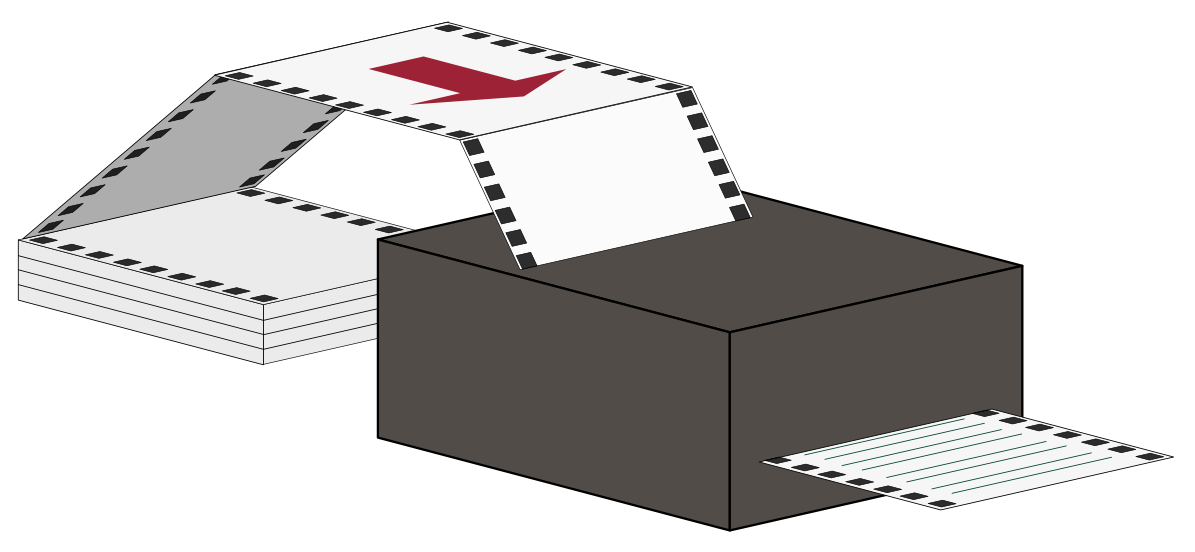
\includegraphics[width=0.4\textwidth]{sprint.png}
      %   \caption{An older, continuous feed printer.}
      %   \label{fig:spec:sem:sprint}
      % \end{figure}

      % \begin{figure}
      %   \centering
      %   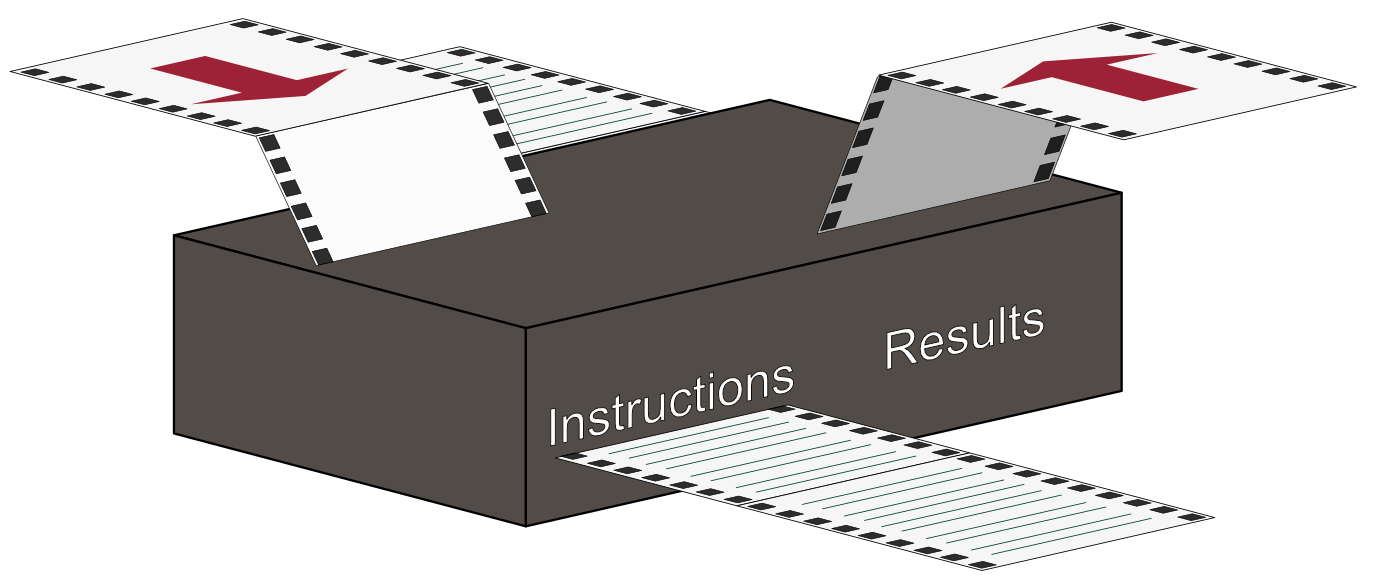
\includegraphics[width=0.4\textwidth]{dprint.png}
      %   \caption{The monitor used in \oldname, demonstrated as a printer operating on two continuous feeds of paper.}
      %   \label{fig:spec:sem:dprint}
      % \end{figure}

      %%%%%%%%%%%%%%%%%%%%%%%%%%%%%
      %%% BEGIN 2SUBSEC 3.2.1   %%%
      %%% SEMANTICS: PREDICATES %%%
      %%%%%%%%%%%%%%%%%%%%%%%%%%%%%
      \subsubsection{Semantics of Predicates}\label{sec:spec:sem:pred}
        This section studies the Semantics of the predicates.
        Please refer to Figure~\ref{fig:spec:sem:pred} for the definitions.
        Note that the \shdtt{$\defeq$} symbol means \textit{``is defined to be equal to''}.
        So, \shdtt{$\interp{abc}\defeq jkl$} can be read as \textit{``The interpretation of abc is definition equivalent to jkl''}.
        % Also, the term \textit{es} in this section refers to when either stream enters the monitor.
        % This is not to be confused with the actual \textit{instruction} stream, which becomes relevant when we discuss the policies in Section~\ref{sec:spec:sem:pol}.

        \paragraph{Falsity:}
          \shdtt{$\interp{ 0 }(-, -)$} \par
          The falsity predicate simply returns nothing.
          There are no possible ins that can satisfy a policy of this nature.

        \paragraph{Identity:}
          \shdtt{$\interp{ 1 }(\mathit{es}, \mathit{ms})$} \par
          The identity is satisfied by every possible input, and therefore returns everything.
          Any instructions or results sent through this monitor pass through completely unaltered.
          The power set of the alphabet is also definition equivalent to the interpretation of Identity.

        \paragraph{Test:}
          \shdtt{$\interp{ f=n }(\mathit{es}, \mathit{ms})$} \par
          The test predicate is satisfied like an \shdtt{if} statement.
          Whenever this statement is satisfied, the policy composed of a test is also satisfied.
          Therefore, a monitor with a test lets all ins pass through which satisfy the given test.
        
        \paragraph{Sum:}
          \shdtt{$\interp{ a + b }(\mathit{es}, \mathit{ms})$} \par
          The sum predicate operates in the same way as the boolean operator.
          For any policy summing two predicates, the inputs that satisfy a, b, or a \textit{and} b are considered to satisfy the entire predicate.
          These ins are passed through the monitor unchanged.
 
        \paragraph{Product:}
          \shdtt{$\interp { a \cdot b }(\mathit{es}, \mathit{ms})$} \par
          As with the sum predicate, the product operator acts like its boolean equivalent.
          Whenever both a \textit{and} b are satisfied, the policy is satisfied.
          Is which satisfy both a and b are passed through the monitor, while all others are ignored.

        \paragraph{Negation:}
          \shdtt{$\interp { \neg a }(\mathit{es}, \mathit{ms})$} \par
          Negation is the final predicate to be examined.
          It is satisfied whenever the argument, a, is not.
          The negation of the identity would therefore return the falsity: \shdtt{$\interp{ \neg 1 }\defeq \interp{0}$}.

        % Semantics of Predicates
        \begin{figure}
          \centering
          { %\fontsize{8pt}{10pt}
          \begin{align*}
            % Theory
            \interp{ \cdot }\ 
              :\ \ &
              \mathbf{Stream}(E)\times \mathbf{Stream}(M) \rightarrow \\
              & P(\mathbf{Stream}(E))\times P(\mathbf{Stream}(M)) 
              \\\hline
            % Falsity
            \interp{ 0 }(-, -)
              \triangleq\ &
              (\emptyset , \emptyset)
              \\ % or null-stream?
            % Identity
            \interp{ 1 }(es, ms)
              \triangleq\ &
              (\{es\},\{ms\})
              \\
            % Test
            \interp{ f=n }(es, ms)
              \triangleq\ &
                (\mathsf{filter}\ (f=n)\ \{es\},\\
              &\ \mathsf{filter}\ (f=n)\ \{ms\}) 
              \\
            % Sum
            \interp{ a + b }(es, ms)
              \triangleq\ &
              \interp { a }(es, ms)\cup
              \interp { b }(es, ms) \\
              &\mathsf{where}\ 
                (S_e^1, S_m^1)\cup (S_e^2, S_m^2)\triangleq\\
                &\quad\quad\ \ \ 
                (S_e^1\cup S_e^2, S_m^1\cup S_m^2)\\
            % Product
            \interp { a \cdot b }(es, ms)
              \triangleq\ &
              \interp { a }(es, ms)\cap
              \interp { b }(es, ms) \\
              &\mathsf{where}\ 
                (S_e^1, S_m^1)\cap (S_e^2, S_m^2)\triangleq\\
                &\quad\quad\ \ \ 
                (S_e^1\cap S_e^2, S_m^1\cap S_m^2)\\
            % Negation
            \interp { \neg a }(es, ms)
              \triangleq\ &
              \mathsf{let}\ (S_e, S_m) = \interp {a}(es, ms) \\
              &\mathsf{in}\ (\{es\} - S_e, \{ms\} - S_m)
              \\
          \end{align*}}
          \caption{The semantics of predicates in \sysname.  While predicates remain unchanged from \oldname, the theory changes slightly}
          \label{fig:spec:sem:pred}
        \end{figure}
      %%%%%%%%%%%%%%%%%%%%%%%%%%%%%
      %%% END 2SUBSEC 3.2.1     %%%
      %%% SEMANTICS: PREDICATES %%%
      %%%%%%%%%%%%%%%%%%%%%%%%%%%%%

      %%%%%%%%%%%%%%%%%%%%%%%%%%%
      %%% BEGIN 2SUBSEC 3.2.2 %%%
      %%% SEMANTICS: POLICIES %%%
      %%%%%%%%%%%%%%%%%%%%%%%%%%%
      \subsubsection{Semantics of Policies:}\label{sec:garuda:sem:pol}
        For policy semantics, it is important to acknowledge the differences between the execution and memory streams.
        These are denoted by \shdtt{$\mathbf{Stream}(E)$} and \shdtt{$\mathbf{Stream}(M)$} respectively.
        \shdtt{$S_e$} and \shdtt{$S_m$} are simply the sets of all in/outs for each stream.
        Refer to Figure~\ref{fig:garuda:sem:pol} for the mathematical definitions.


        \paragraph{Injection to State Register:}
          \shdtt{$\interp { inj_{i}(i) }(\mathit{es}, \mathit{ms})$} \par
          Injection to State Register will inject an instruction into the stream.
          Imagine if the printer could add its own page to the middle of a multi-page job.
          This is pretty much the same as what injecting a value does.
          The injected data are not in the input stream for the instructions, but appears on the output.

        \paragraph{Injection to Memory Unit:}
          \shdtt{$\interp { inj_{r}(r) }(\mathit{es}, \mathit{ms})$} \par
          Injecting to the memory unit acts the same as injecting data to the state register.
          Rather, it injects on the register-to-memory stream.


        \paragraph{Modification:}
          \shdtt{$\interp { f \leftarrow n }(\mathit{es}, \mathit{ms})$} \par
          Modification is \sysname's system for assigning a variable, or field.
          Modification can be used if the programmer would like to redirect a sensitive result to a secure address.
          It can also be used to temporarily store a value to be re-inserted later.

        \paragraph{Policy Union:}
          \shdtt{$\interp { p + q }(\mathit{es}, \mathit{ms})$} \par
          A policy union is when a programmer wishes to have two separare policies operate in parallel.
          Often times, only the $p$ or $q$ policies are satisfied, and not both.
          This can be used in decision making or if the user wants to apply one policy to the results and a different one to the actions.
          In this case, they would also use the slicing rules.

        \paragraph{Policy Concatenation:}
          \shdtt{$\interp { p \cdot q }(\mathit{es}, \mathit{ms})$} \par
          Policy concatenation is used when the user wants to design a policy that has specific prerequisites to trigger.
          A policy may modify all branches, but only \textit{after} a load instruction has passed through.
          This allows for a granular, state-machine-like implementation of multiple policies at once.


        \paragraph{Filter:}
          \shdtt{$\interp{\mathsf{filter}\ f}(S)$} \par
          The filter is a function defined to assist in describing the semantics of test.
          It is included at the end of policy syntax definitions, as it also applies to the use of ``test'' as a policy.
          While the keyword is never used, the test policy functions the same as the test predicate.
          Filter is explained by its namesake.
          It is an operation over a set $S$ which returns all elements that satisfy the conditional $f$.

        \paragraph{Map:}
          \shdtt{$\interp{\mathsf{map}\ g}(S)$} \par
          The map is very similar to the filter.
          Unlike filter, which takes a conditional $f$, map takes a function $g$.
          This function is applied to all elements in the set $S$, returning a modified set $S'$.

      \subsubsection{Semantics of Policies}\label{sec:spec:sem:pol}
        \begin{figure}
          \centering
          { %\fontsize{8}{10}
          \begin{align*}
            % Theory
            \interp { \cdot }\ 
              :\ \ &
              \mathbf{Stream}(E)\times \mathbf{Stream}(M) \rightarrow \\
              & P(\mathbf{Stream}(E))\times P(\mathbf{Stream}(M)) 
              \\\hline
            % Obfuscation
            \interp {(\Phi_{En}, \Phi_{De})}(es, ms)\
              \triangleq\
              & \mathsf{let}\ (e \rightarrow \obf{e} = \Phi_{En}),\\
              & \quad\ \      (\obf{m} \rightarrow m = \Phi_{De}) \\
              % & \mathsf{let}\ e \rightarrow \obf{e} = \Phi_{Encrypt}\\
              % & \mathsf{and}\ \obf{m} \rightarrow m = \Phi_{Decrypt}\\
              & \mathsf{in}\
              (\{\obf{e}\}, \{m\})
              \\
            % Injection to State Register
            \interp { inj_{SR}(e) }(es, ms)
              \triangleq\ &
              (\{e : es\}, \{ms\}) 
              % or ::?  ;i sequential
              \\
            % Injection to Memory Unit
            \interp { inj_{Mi}(m) }(es, ms)
              \triangleq\ &
              (\{es\},\{m : ms\})
              \\
            % Modification
            \interp { f \leftarrow n }(es, ms)
              \triangleq\ 
              & (\mathsf{map}\ (f\leftarrow n)\ \{e\},\\
              &\ \mathsf{map}\ (f\leftarrow n)\ \{m\})
              \\ %  could use editing?
            % Policy Union
            \interp { p + q }(es, ms)
              \triangleq\ &
              \interp { p }(e, m)\cup
              \interp { q }(e, m) \\
              &\mathsf{where}\ (S_e^1, S_m^1)\cup (S_e^2, S_m^2)\triangleq\\
              &\quad\quad\quad (S_e^1\cup S_e^2, S_m^1\cup S_m^2)\\
              % A union of the streams gives a nondeterministic machine.
            % Policy Concatnation
            \interp { p \cdot q }(es, ms)
              \triangleq\ &
              \mathsf{let}\ (S_e, S_m) = \interp{p}(e, m)\\
              &\mathsf{in}\ \bigcup \{\interp{q}(e',m')\ |\ e'\in S_e, m'\in S_m\}\\
              % \\
              \hline
            % Defn. of Filter
            \interp{\mathsf{filter}\ f}(S)
              \triangleq\ & \{l \in S\ |\ f(l) = \mathsf{true}\}\\
            % Defn. of Map
            \interp{\mathsf{map}\ g}(S)
              \triangleq\ &
              \{ g(l)\ |\ l\in S \} 
          \end{align*}}
          \caption{The semantics of policies in \sysname.}
          \label{fig:spec:sem:pol}
        \end{figure}
    %}
  %%%%%%%%%%%%%%%%%%%%%%%%%%%%%
  %%% END OF SUBSECTION 3.2 %%%
  %%% SYSTEM SEMANTICS      %%%
  %%%%%%%%%%%%%%%%%%%%%%%%%%%%%

  %%%%%%%%%%%%%%%%%%%%%%%%%%%%%%%
  %%% BEGIN OF SUBSECTION 3.3 %%%
  %%% SYSTEM LIMITATIONS      %%%
  %%%%%%%%%%%%%%%%%%%%%%%%%%%%%%%
    \subsection{The Limitations of \sysname}\label{sec:spec:lim}
      The \sysname language was designed to be as expressive as possible, but some of our defining characteristics have their inherent flaws.
      To start, \sysname assumes a single-stream in and single-stream out model.
      This means that it is not possible to send multiple instructions at once, like in VLIW\footnote{
      Very Long Instruction Word: refers to the idea of packing multiple standard instructions into a single machine command.} or thread-parallel processors.
      Non-sequential instructions pose an issue as well; \sysname is not equipped to handle multiple outputs at once.
      This presents a bottleneck to the results stream.
      Out-of-Order Execution is, therefore, not currently supported in an efficient way\footnote{See Section~\ref{sec:more:ooe} for more discussion on my attempts to remedy this.}.
      \par

      \sysname is also not programmable after synthesis.
      It may be possible to cleverly design a dynamic policy to handle a wide range of cases and interpret the situation is presented intelligently.
      Still, an unforeseen edge case can not be added after compiling this policy.
      To make something programmable, an engineer would have to settle for a \textit{Field Programmable Gate Array} (FPGA).
      These devices tend to be a lot less efficient than on-chip designs, as they are (almost) always found outside the processor package.
      \par

      There are a few limitations of the compiler as well.
      I leave the discussion of lower-level limitations for Section~\ref{sec:compile:lim}.
%%%%%%%%%%%%%%%%%%%%%%%%
%%% END OF SECTION 3 %%%
%%% GARUDA SPECIFICS %%%
%%%%%%%%%%%%%%%%%%%%%%%%
%%%%%%%%%%%%%%%%%%%%%%
%%% BEGIN SECTON 4 %%%
%%% PROOFS         %%%
%%%%%%%%%%%%%%%%%%%%%%
  \section{TODO (Name): Proofs}\label{sec:proofs}
    %%%%%%%%%%%%%%%%%%%%%%%%
    %%% BEGIN SECTON 4.0 %%%
    %%% WHY PROOFS       %%%
    %%%%%%%%%%%%%%%%%%%%%%%%

    %%%%%%%%%%%%%%%%%%%%%%%%
    %%% BEGIN SECTON 4.1 %%%
    %%% NO OBFUSCATION   %%%
    %%%%%%%%%%%%%%%%%%%%%%%%
    %%% Demonstrate the basic flow of a policy

    %%%%%%%%%%%%%%%%%%%%%%%%
    %%% BEGIN SECTON 4.2 %%%
    %%% XOR KEY          %%%
    %%%%%%%%%%%%%%%%%%%%%%%%
    %%% Demonstrate proofs on converse PhiOps

    %%%%%%%%%%%%%%%%%%%%%%%%
    %%% BEGIN SECTON 4.3 %%%
    %%% SOMETHING ABOUT PHI STACKING ??? %%%
    %%%%%%%%%%%%%%%%%%%%%%%%
    %%% Demonstrate complex policy decision making


    %%%%%%%%%%%%%%%%%%%%%%%%
    %%% BEGIN SECTON 4.1 %%%
    %%% EXAMPLE ATTACKS  %%%
    %%%%%%%%%%%%%%%%%%%%%%%%
    %%% Demonstrate a thwarted attack

%%%%%%%%%%%%%%%%%%%%%%%%
%%% BEGIN SECTON 5   %%%
%%% FULL COMPILATION %%%
%%%%%%%%%%%%%%%%%%%%%%%%
  \section{Compilation to Verilog}\label{sec:comp}
    %%%%%%%%%%%%%%%%%%%%%%%%
    %%% BEGIN SECTON 5.1 %%%
    %%% INTERMEDIATE     %%%
    %%%%%%%%%%%%%%%%%%%%%%%%
    \subsection{The Intermediate Language}\label{sec:comp:int}

      \begin{figure}
        \centering
        \begin{tabular}{l r r l l}
          % Definitions table
          Values        & $v$     & $::=$     & $\mathsf{INSTR\ |\ RES}$ &\\
          Registers     & $b$     & $::=$     & $\mathsf{reg}$           &\\
          \\
          % Predicates table
          Expressions & $e$ & $::=$  & $read(b)$       
                            & \textit{Read Reg}\\
                      &     & $\mid$ & $write(b,v)$    
                            & \textit{Write Value to Reg}\\
                      &     & $\mid$ & $let\ x = e_1\ in\ e_2$ 
                            & \textit{Assignment}\\  
                      &     & $\mid$ & $e_1\ ||\ e_2$ 
                            & \textit{Parallel}\\
                      &     & $\mid$ & $f(e_1)$        
                            & \textit{Apply Function} \\  
                      &     & $\mid$ & $if\ v = n\ then\ e_1\ else\ e_2$
                            & \textit{Conditional} \\
                      &     & $\mid$ & $e_1\ \&\&\ e_2$ 
                            & \textit{Product (AND)}\\
                      &     & $\mid$ & $e_1 ; e_2$
                            & \textit{Concatenation}\\
                      &     & $\mid$ & $forever\ e$ 
                            & \textit{Hardwire}
        \end{tabular}
        \caption{The language \sysname uses as a means to facilitate compilation.}
        \label{fig:comp:int}
      \end{figure}
    %%%%%%%%%%%%%%%%%%%%%%%%
    %%% BEGIN SECTON 5.2 %%%
    %%% COMPILATION      %%%
    %%%%%%%%%%%%%%%%%%%%%%%%
    \subsection{Compiling \sysname to the Intermediate}\label{sec:comp:comp}
      We define a function $\mathbf{C}$ to be the compilation of some predicate or policy in \sysname to the intermediate language.
      $\mathbf{C}$ operates on the four ports of the \sysname monitor.
      These consist of the processing done after the Execution stage, before the Memory stage, and their respective altered streams.
      Table~\ref{tab:compile:compile:ports} summarizes each port.
      Assume all $\mathbf{C}$ are short for $\mathbf{C}_{(EXE,\obf{EXE},\obf{MEM},MEM)}$ if unspecified.
      % Would it be best to flip MEM and MEM' to show the return to the original output of EXE?
      \begin{table}
        \centering
        \begin{tabular}{c | l}
          PORT        & DESCRIPTION \\ \hline
          $EXE$       & Direct output of the execution stage. \\
          $\obf{EXE}$ & Altered state register input. \\
          $\obf{MEM}$ & Direct output of the state register. \\
          $MEM$       & Altered memory access input. 
        \end{tabular}
        \caption{
          The four ports used in compilation.
          These are the inputs and outputs for logic between the functional units and state register.
        }
        \label{tab:comp:comp:ports}
      \end{table}

      %%%%%%%%%%%%%%%%%%%%%%%%%%
      %%% BEGIN SECTON 5.2.1 %%%
      %%% PREDICATES         %%%
      %%%%%%%%%%%%%%%%%%%%%%%%%%
      \subsubsection{Compiling Predicates}\label{sec:comp:comp:pred}
        \begin{figure}
          \begin{align*}
            % Falsity
            \mathbf{C}[0]\ 
              =\ &
              let\    E\_bog = \text{new buf}\\
              &\quad\ M\_bog = \text{new buf}\\
              &in\ write(\obf{EXE}, E\_bog)\\
              &\quad  write(MEM, M\_bog)\\
            % Identity
            \mathbf{C}[1]\ 
              =\ &
              write(\obf{EXE}, read(EXE))\\
              &write(MEM, read(\obf{MEM}))
              \\
            % Filter
            \mathbf{C}[f = n]\
              =\
              &if\ EXE=n\ then\\
              &\quad write(\obf{EXE}, read(EXE))\\
              &\quad else\ \mathbf{C}_{(EXE, \obf{EXE}, -, -)}[0]\\
              &if\ \obf{MEM}=n\ then\\
              &\quad write(MEM, read(\obf{MEM}))\\
              &\quad else\ \mathbf{C}_{(-, -, \obf{MEM}, MEM)}[0]\\
            % Predicate Addition
            \mathbf{C}[\mathsf{test}(a + b)]\ 
              =\
              & (*Intermediate\ Execution\ Ports*)\\
              & let\ E_{ai}, \obf{E}_{ai}, E_{bi}, \obf{E}_{bi} = \text{new buf}\ in\\
              & (*Intermediate\ Memory\ Ports*)\\
              & let\ \obf{M}_{ai}, M_{ai}, \obf{M}_{bi}, M_{bi} = \text{new buf}\ in\\
              &\quad\ \ DeMux(EXE, E_{ai}, E_{bi})\ ||\\
              &\quad\ \ DeMux(\obf{MEM}, \obf{M}_{ai}, \obf{M}_{bi})\\
              &let\     i_a = \mathbf{C}_{(E_{ai},\obf{E}_{ai},\obf{M}_{ai},M_{ai})}[a]\\
              &\quad\ \ i_b = \mathbf{C}_{(E_{bi},\obf{E}_{bi},\obf{M}_{bi},M_{bi})}[b]\\
              &in\ Mux(i_a\ \ i_b, (\obf{EXE},MEM))\\
            % Predicate Product
            \mathbf{C}[\mathsf{test}(a \cdot b)]\ 
              =\ &\mathbf{C}[\mathsf{test}(a) \cdot \mathsf{test}(b)] \\
            % Predicate Negation
            \mathbf{C}[\neg a]\ 
              =\ 
              &if\ \neg a\ then\\
              &\quad write(\obf{EXE}, read(EXE))\\
              &\quad write(MEM, read(\obf{MEM}))\\
              &else\ \mathbf{C}[0]\\
          \end{align*}
          \caption{
            Compilation of \sysname predicates into the intermediate language.
            These remain largely unchanged from \oldname.
          }
          \label{fig:comp:comp:pred}
        \end{figure}

    %%%%%%%%%%%%%%%%%%%%%%%%%%
    %%% BEGIN SECTON 5.2.2 %%%
    %%% POLICIES           %%%
    %%%%%%%%%%%%%%%%%%%%%%%%%%
      \subsubsection{Compiling Policies}\label{sec:comp:comp:pol}
        \begin{figure}
          \begin{align*}
            % Inject Instruction
            \mathbf{C}[inj_{SR}V]\ 
              =\ &
              write(\obf{EXE}, V)\\
            % Inject Result
            \mathbf{C}[inj_{Mi}V]\ 
              =\ &
              write(MEM, V)\\
            % Assignment
            \mathbf{C}[f \leftarrow n]\ 
              =\ &
              let\    e' = f(read(EXE))\\
              &\quad\ m' = f(read(\obf{MEM}))\\
              &in\ write(\obf{EXE}, e')\\
              &\quad \ write(MEM, m')\\
            % Policy Nondeterministic Choice
            \mathbf{C}[p + q]\ 
              =\ &
              let\      e_p = \mathbf{C}[p]\\
              &\quad\ \ e_q = \mathbf{C}[q]\\
              &in\ Mux(e_p, e_q, (\obf{EXE},MEM))\\
            % Policy Sequence
            \mathbf{C}[p \cdot q]\ 
              =\ &
              let\    EXE_{mid} = \text{new buf}\\
              &\quad\ MEM_{mid} = \text{new buf}\\
              &\quad\ \ e_p = \mathbf{C}_{( EXE, EXE_{mid}, \obf{MEM}, MEM_{mid}      )}[p]\\
              &\quad\ \ e_q = \mathbf{C}_{(      EXE_{mid}, \obf{EXE}, MEM_{mid}, MEM )}[q]\\
              &in\ e_p\ ;\ e_q
          \end{align*}
          \caption{Compilation of \sysname policies into the intermediate language.}
          \label{fig:comp:comp:pol}
        \end{figure}





%%
%% The acknowledgments section is defined using the "acks" environment
%% (and NOT an unnumbered section). This ensures the proper
%% identification of the section in the article metadata, and the
%% consistent spelling of the heading.
\begin{acks}
To ...
\end{acks}

%%
%% The next two lines define the bibliography style to be used, and
%% the bibliography file.
\bibliographystyle{ACM-Reference-Format}
\bibliography{Garuda2.0}

%%
%% If your work has an appendix, this is the place to put it.
\appendix

\section{Research Methods}

\subsection{Part One}

Appendix A1

\subsection{Part Two}

Appendix A2

\section{Online Resources}

Appendix B

\end{document}
\endinput
